% Options for packages loaded elsewhere
\PassOptionsToPackage{unicode}{hyperref}
\PassOptionsToPackage{hyphens}{url}
%
\documentclass[
]{article}
\usepackage{amsmath,amssymb}
\usepackage{iftex}
\ifPDFTeX
  \usepackage[T1]{fontenc}
  \usepackage[utf8]{inputenc}
  \usepackage{textcomp} % provide euro and other symbols
\else % if luatex or xetex
  \usepackage{unicode-math} % this also loads fontspec
  \defaultfontfeatures{Scale=MatchLowercase}
  \defaultfontfeatures[\rmfamily]{Ligatures=TeX,Scale=1}
\fi
\usepackage{lmodern}
\ifPDFTeX\else
  % xetex/luatex font selection
\fi
% Use upquote if available, for straight quotes in verbatim environments
\IfFileExists{upquote.sty}{\usepackage{upquote}}{}
\IfFileExists{microtype.sty}{% use microtype if available
  \usepackage[]{microtype}
  \UseMicrotypeSet[protrusion]{basicmath} % disable protrusion for tt fonts
}{}
\makeatletter
\@ifundefined{KOMAClassName}{% if non-KOMA class
  \IfFileExists{parskip.sty}{%
    \usepackage{parskip}
  }{% else
    \setlength{\parindent}{0pt}
    \setlength{\parskip}{6pt plus 2pt minus 1pt}}
}{% if KOMA class
  \KOMAoptions{parskip=half}}
\makeatother
\usepackage{xcolor}
\usepackage[margin=1in]{geometry}
\usepackage{color}
\usepackage{fancyvrb}
\newcommand{\VerbBar}{|}
\newcommand{\VERB}{\Verb[commandchars=\\\{\}]}
\DefineVerbatimEnvironment{Highlighting}{Verbatim}{commandchars=\\\{\}}
% Add ',fontsize=\small' for more characters per line
\usepackage{framed}
\definecolor{shadecolor}{RGB}{248,248,248}
\newenvironment{Shaded}{\begin{snugshade}}{\end{snugshade}}
\newcommand{\AlertTok}[1]{\textcolor[rgb]{0.94,0.16,0.16}{#1}}
\newcommand{\AnnotationTok}[1]{\textcolor[rgb]{0.56,0.35,0.01}{\textbf{\textit{#1}}}}
\newcommand{\AttributeTok}[1]{\textcolor[rgb]{0.13,0.29,0.53}{#1}}
\newcommand{\BaseNTok}[1]{\textcolor[rgb]{0.00,0.00,0.81}{#1}}
\newcommand{\BuiltInTok}[1]{#1}
\newcommand{\CharTok}[1]{\textcolor[rgb]{0.31,0.60,0.02}{#1}}
\newcommand{\CommentTok}[1]{\textcolor[rgb]{0.56,0.35,0.01}{\textit{#1}}}
\newcommand{\CommentVarTok}[1]{\textcolor[rgb]{0.56,0.35,0.01}{\textbf{\textit{#1}}}}
\newcommand{\ConstantTok}[1]{\textcolor[rgb]{0.56,0.35,0.01}{#1}}
\newcommand{\ControlFlowTok}[1]{\textcolor[rgb]{0.13,0.29,0.53}{\textbf{#1}}}
\newcommand{\DataTypeTok}[1]{\textcolor[rgb]{0.13,0.29,0.53}{#1}}
\newcommand{\DecValTok}[1]{\textcolor[rgb]{0.00,0.00,0.81}{#1}}
\newcommand{\DocumentationTok}[1]{\textcolor[rgb]{0.56,0.35,0.01}{\textbf{\textit{#1}}}}
\newcommand{\ErrorTok}[1]{\textcolor[rgb]{0.64,0.00,0.00}{\textbf{#1}}}
\newcommand{\ExtensionTok}[1]{#1}
\newcommand{\FloatTok}[1]{\textcolor[rgb]{0.00,0.00,0.81}{#1}}
\newcommand{\FunctionTok}[1]{\textcolor[rgb]{0.13,0.29,0.53}{\textbf{#1}}}
\newcommand{\ImportTok}[1]{#1}
\newcommand{\InformationTok}[1]{\textcolor[rgb]{0.56,0.35,0.01}{\textbf{\textit{#1}}}}
\newcommand{\KeywordTok}[1]{\textcolor[rgb]{0.13,0.29,0.53}{\textbf{#1}}}
\newcommand{\NormalTok}[1]{#1}
\newcommand{\OperatorTok}[1]{\textcolor[rgb]{0.81,0.36,0.00}{\textbf{#1}}}
\newcommand{\OtherTok}[1]{\textcolor[rgb]{0.56,0.35,0.01}{#1}}
\newcommand{\PreprocessorTok}[1]{\textcolor[rgb]{0.56,0.35,0.01}{\textit{#1}}}
\newcommand{\RegionMarkerTok}[1]{#1}
\newcommand{\SpecialCharTok}[1]{\textcolor[rgb]{0.81,0.36,0.00}{\textbf{#1}}}
\newcommand{\SpecialStringTok}[1]{\textcolor[rgb]{0.31,0.60,0.02}{#1}}
\newcommand{\StringTok}[1]{\textcolor[rgb]{0.31,0.60,0.02}{#1}}
\newcommand{\VariableTok}[1]{\textcolor[rgb]{0.00,0.00,0.00}{#1}}
\newcommand{\VerbatimStringTok}[1]{\textcolor[rgb]{0.31,0.60,0.02}{#1}}
\newcommand{\WarningTok}[1]{\textcolor[rgb]{0.56,0.35,0.01}{\textbf{\textit{#1}}}}
\usepackage{graphicx}
\makeatletter
\def\maxwidth{\ifdim\Gin@nat@width>\linewidth\linewidth\else\Gin@nat@width\fi}
\def\maxheight{\ifdim\Gin@nat@height>\textheight\textheight\else\Gin@nat@height\fi}
\makeatother
% Scale images if necessary, so that they will not overflow the page
% margins by default, and it is still possible to overwrite the defaults
% using explicit options in \includegraphics[width, height, ...]{}
\setkeys{Gin}{width=\maxwidth,height=\maxheight,keepaspectratio}
% Set default figure placement to htbp
\makeatletter
\def\fps@figure{htbp}
\makeatother
\setlength{\emergencystretch}{3em} % prevent overfull lines
\providecommand{\tightlist}{%
  \setlength{\itemsep}{0pt}\setlength{\parskip}{0pt}}
\setcounter{secnumdepth}{-\maxdimen} % remove section numbering
\usepackage{fvextra}
\DefineVerbatimEnvironment{Highlighting}{Verbatim}{breaklines,commandchars=\\\{\}}
\ifLuaTeX
  \usepackage{selnolig}  % disable illegal ligatures
\fi
\usepackage{bookmark}
\IfFileExists{xurl.sty}{\usepackage{xurl}}{} % add URL line breaks if available
\urlstyle{same}
\hypersetup{
  pdftitle={SDA Group Submission Assignment Assign1},
  pdfauthor={MengliFeng (2720589) and PepijnVanOostveen (2801582)},
  hidelinks,
  pdfcreator={LaTeX via pandoc}}

\title{SDA Group Submission Assignment Assign1}
\usepackage{etoolbox}
\makeatletter
\providecommand{\subtitle}[1]{% add subtitle to \maketitle
  \apptocmd{\@title}{\par {\large #1 \par}}{}{}
}
\makeatother
\subtitle{Group Gr18}
\author{MengliFeng (2720589) and PepijnVanOostveen (2801582)}
\date{}

\begin{document}
\maketitle

\section{Exercise 1}\label{exercise-1}

\subsection{a.}\label{a.}

\begin{Shaded}
\begin{Highlighting}[]
\CommentTok{\# Step 1: Create the contingency matrix}
\NormalTok{email\_matrix }\OtherTok{\textless{}{-}} \FunctionTok{matrix}\NormalTok{(}\FunctionTok{c}\NormalTok{(}\DecValTok{9}\NormalTok{, }\DecValTok{11}\NormalTok{, }\DecValTok{4}\NormalTok{, }\DecValTok{21}\NormalTok{), }\AttributeTok{nrow =} \DecValTok{2}\NormalTok{, }\AttributeTok{byrow =} \ConstantTok{FALSE}\NormalTok{,}
                       \AttributeTok{dimnames =} \FunctionTok{list}\NormalTok{(}\AttributeTok{Spam\_Status =} \FunctionTok{c}\NormalTok{(}\StringTok{"Spam"}\NormalTok{, }\StringTok{"Not\_Spam"}\NormalTok{),}
                                       \AttributeTok{Urgency =} \FunctionTok{c}\NormalTok{(}\StringTok{"Urgent"}\NormalTok{, }\StringTok{"Not\_Urgent"}\NormalTok{)))}

\CommentTok{\# Step 2: Mosaic plot with custom colors}
\FunctionTok{mosaicplot}\NormalTok{(email\_matrix, }\AttributeTok{color =} \FunctionTok{c}\NormalTok{(}\StringTok{"tomato"}\NormalTok{, }\StringTok{"lightblue"}\NormalTok{), }
           \AttributeTok{main =} \StringTok{"Mosaic Plot of Email Spam by Urgency"}\NormalTok{,}
           \AttributeTok{xlab =} \StringTok{"Urgency"}\NormalTok{, }\AttributeTok{ylab =} \StringTok{"Spam Status"}\NormalTok{, }
           \AttributeTok{sort =} \DecValTok{1}\SpecialCharTok{:}\DecValTok{2}\NormalTok{, }\AttributeTok{dir =} \FunctionTok{c}\NormalTok{(}\StringTok{"h"}\NormalTok{, }\StringTok{"v"}\NormalTok{))}
\end{Highlighting}
\end{Shaded}

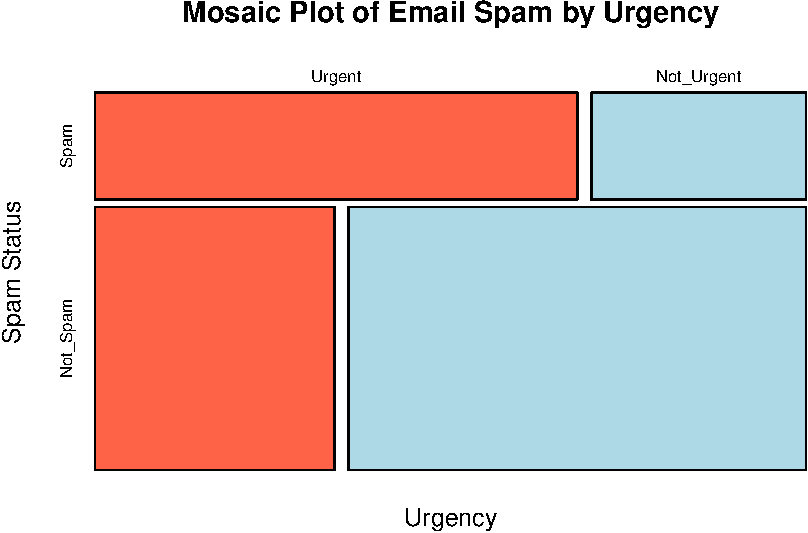
\includegraphics{SDA_A6_files/figure-latex/unnamed-chunk-1-1.pdf}

\subsection{b.}\label{b.}

P(Spam\textbar Urgent) = 9/(9+4) = 0.692 this is computed by diving the
number of spam labeled urgent and the total emails that are labeled as
urgent.

\subsection{c.}\label{c.}

\begin{Shaded}
\begin{Highlighting}[]
\CommentTok{\# Extract values}
\NormalTok{a }\OtherTok{\textless{}{-}}\NormalTok{ email\_matrix[}\StringTok{"Spam"}\NormalTok{, }\StringTok{"Urgent"}\NormalTok{]}
\NormalTok{b }\OtherTok{\textless{}{-}}\NormalTok{ email\_matrix[}\StringTok{"Not\_Spam"}\NormalTok{, }\StringTok{"Urgent"}\NormalTok{]}
\NormalTok{c }\OtherTok{\textless{}{-}}\NormalTok{ email\_matrix[}\StringTok{"Spam"}\NormalTok{, }\StringTok{"Not\_Urgent"}\NormalTok{]}
\NormalTok{d }\OtherTok{\textless{}{-}}\NormalTok{ email\_matrix[}\StringTok{"Not\_Spam"}\NormalTok{, }\StringTok{"Not\_Urgent"}\NormalTok{]}

\CommentTok{\# Compute conditional probabilities}
\NormalTok{odds\_ratio }\OtherTok{\textless{}{-}}\NormalTok{ (a }\SpecialCharTok{/}\NormalTok{ b) }\SpecialCharTok{/}\NormalTok{ (c }\SpecialCharTok{/}\NormalTok{ d)}
\NormalTok{odds\_ratio}
\end{Highlighting}
\end{Shaded}

\begin{verbatim}
## [1] 4.295455
\end{verbatim}

\subsection{d.}\label{d.}

\begin{Shaded}
\begin{Highlighting}[]
\CommentTok{\# Perform one{-}sided Fisher\textquotesingle{}s exact test}
\NormalTok{fisher\_result }\OtherTok{\textless{}{-}} \FunctionTok{fisher.test}\NormalTok{(email\_matrix, }\AttributeTok{alternative =} \StringTok{"greater"}\NormalTok{)}
\NormalTok{fisher\_result}
\end{Highlighting}
\end{Shaded}

\begin{verbatim}
## 
##  Fisher's Exact Test for Count Data
## 
## data:  email_matrix
## p-value = 0.03566
## alternative hypothesis: true odds ratio is greater than 1
## 95 percent confidence interval:
##  1.107161      Inf
## sample estimates:
## odds ratio 
##   4.148314
\end{verbatim}

since we want to know if urgent means more likely spam (not just
related), we use one-sided test, with alternative odds is greater than 1
(urgent emails have higher odds being spam). the null is rejected

\section{Exercise 2}\label{exercise-2}

\subsection{a.}\label{a.-1}

\begin{Shaded}
\begin{Highlighting}[]
\CommentTok{\# Create the table and then use it to make a mosaicplot}
\NormalTok{titanic\_CS }\OtherTok{\textless{}{-}} \FunctionTok{margin.table}\NormalTok{(Titanic, }\AttributeTok{margin =} \FunctionTok{c}\NormalTok{(}\DecValTok{1}\NormalTok{, }\DecValTok{4}\NormalTok{))}
\FunctionTok{mosaicplot}\NormalTok{(titanic\_CS, }\AttributeTok{main =} \StringTok{"Titanic Survival by Class"}\NormalTok{, }\AttributeTok{color =} \FunctionTok{c}\NormalTok{(}\StringTok{"red"}\NormalTok{, }\StringTok{"darkgreen"}\NormalTok{))}
\end{Highlighting}
\end{Shaded}

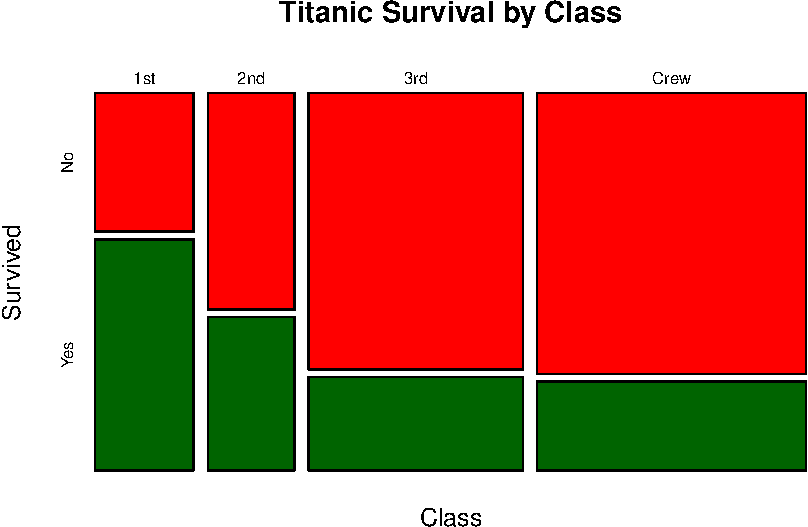
\includegraphics{SDA_A6_files/figure-latex/unnamed-chunk-4-1.pdf} There
is an obvious correlation between the class and chance of survival. So
the wealthier you were (or more accurately the more you spent on your
ticket) the likelier you were to survive with the crew being the least
likely to survive.

\subsection{b.}\label{b.-1}

\begin{Shaded}
\begin{Highlighting}[]
\CommentTok{\# Do the test}
\FunctionTok{chisq.test}\NormalTok{(titanic\_CS)}
\end{Highlighting}
\end{Shaded}

\begin{verbatim}
## 
##  Pearson's Chi-squared test
## 
## data:  titanic_CS
## X-squared = 190.4, df = 3, p-value < 2.2e-16
\end{verbatim}

The p-value is less than 10\^{}-15 it is far smaller than the
significance level of 0.05 and thus the null is rejected as we expected.
This means that the test had the same result as we had by just looking
at the mosaic namely that there is a relationship between the class and
the chance to survive.

\subsection{c.}\label{c.-1}

\begin{Shaded}
\begin{Highlighting}[]
\CommentTok{\# Get the expected values}
\NormalTok{test\_result }\OtherTok{\textless{}{-}} \FunctionTok{chisq.test}\NormalTok{(titanic\_CS)}
\NormalTok{test\_result}\SpecialCharTok{$}\NormalTok{expected}
\end{Highlighting}
\end{Shaded}

\begin{verbatim}
##       Survived
## Class        No       Yes
##   1st  220.0136 104.98637
##   2nd  192.9350  92.06497
##   3rd  477.9373 228.06270
##   Crew 599.1140 285.88596
\end{verbatim}

\begin{Shaded}
\begin{Highlighting}[]
\CommentTok{\# The real values}
\NormalTok{titanic\_CS}
\end{Highlighting}
\end{Shaded}

\begin{verbatim}
##       Survived
## Class   No Yes
##   1st  122 203
##   2nd  167 118
##   3rd  528 178
##   Crew 673 212
\end{verbatim}

The values that are the farthest apart from the expected values is the
survival chance of 1st class, but I expected that so the thing that I
found most striking is that there is almost no difference between 3rd
class and the crew. I thought that knowing more about the ship would
help the crew and that 3rd class had the lowest chances since 1st and
2nd class were situated better.

\subsection{d.}\label{d.-1}

\begin{Shaded}
\begin{Highlighting}[]
\CommentTok{\# get the 3rd and crew rows from our table}
\NormalTok{third\_crew }\OtherTok{\textless{}{-}}\NormalTok{ titanic\_CS[}\FunctionTok{c}\NormalTok{(}\StringTok{"3rd"}\NormalTok{, }\StringTok{"Crew"}\NormalTok{), ]}

\CommentTok{\# make it a matrix and then test as alternative greater since the first row is 3rd class and we want to know if first class has a better survival chance}
\NormalTok{survival\_table }\OtherTok{\textless{}{-}} \FunctionTok{as.matrix}\NormalTok{(third\_crew)}
\FunctionTok{fisher.test}\NormalTok{(survival\_table, }\AttributeTok{alternative =} \StringTok{"greater"}\NormalTok{)}
\end{Highlighting}
\end{Shaded}

\begin{verbatim}
## 
##  Fisher's Exact Test for Count Data
## 
## data:  survival_table
## p-value = 0.7385
## alternative hypothesis: true odds ratio is greater than 1
## 95 percent confidence interval:
##  0.7657002       Inf
## sample estimates:
## odds ratio 
##  0.9344464
\end{verbatim}

The p-value is 0.7385 so the survival chance isn't significantly higher
for 3rd class and thus the hypothesis that the chacnes are equal isn't
rejected.

\end{document}
